\scanpage{17}
\uline{Cas particuliers}

Supposons que $\forall i\in I$, \deleted{$\unsure{E_i|\Sigma_i}$ \unsure{est|soit} rare dans $X$.} \inserted{on ait} (si $\Sigma_i^+\ \Sigma_i^-$ sont les deux comp. conn. de $X\setminus\Sigma_i$)

\deleted{Alors on \unsure{trouve} que}
\[
\begin{aligned}
\overline{\Sigma_i^+} &= \Sigma_i^+\cup E_i\\
\overline{\Sigma_i^-} &= \Sigma_i^-\cup E_i\hspace{1.5cm}
% M01: source origin (1172,557); observed triangular point, period interpretation retained as alternative.
\mathpunct{\unsure{\begin{tikzpicture}[x=0.01cm,y=-0.01cm,baseline=(monebase)]
\coordinate (monebase) at (0,6);
\path[use as bounding box] (0,0) rectangle (7,7);
\fill (1,5) -- (3,1) -- (5,0) -- (7,5) -- cycle;
\end{tikzpicture}|.}}
\end{aligned}
\]

Alors je dis qu'on a
\[
\overline{\Sigma_{12}}=\Sigma_{12}
% G01: source origin (947,783); literal retraced cup; source alternative amalg is retained in the decision record.
\mathbin{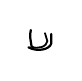
\begin{tikzpicture}[x=0.01cm,y=-0.01cm,baseline=(joinbase)]
\coordinate (joinbase) at (0,29);
\path[use as bounding box] (0,0) rectangle (33,32);
\draw[line width=0.8pt,line cap=round] (4,3) .. controls (2,10) and (4,17) .. (5,24);
\draw[line width=0.65pt,line cap=round] (5,24) .. controls (12,28) and (25,24) .. (25,17) -- (22,7);
\draw[line width=0.8pt,line cap=round] (1,25) .. controls (12,31) and (28,28) .. (30,20) -- (30,8);
\end{tikzpicture}}E_1\cup E_2
\]

% G02: dividing rule; source origin (300,887). The wide fixed rectangle retains its left placement.
\figure{\begin{tikzpicture}[x=0.01cm,y=-0.01cm]
\path[use as bounding box] (0,0) rectangle (1300,25);
\draw[line width=0.3pt,line cap=round] (2,14) .. controls (40,6) and (105,11) .. (145,8) .. controls (183,6) and (222,4) .. (237,8) .. controls (239,9) and (237,12) .. (239,13);
\end{tikzpicture}}

% slanted
\reversemarginpar
\margin{introduire la partition $\unsure{\Pi|\pi}_j=\{\deleted{\unsure{\Sigma}}E_j,\Sigma_j^+,\Sigma_j^-\}$}
\normalmarginpar
\deleted{Supposons}

Soit $J\subset I$ tel que $I=J\amalg\{i\}$.

Considerons la partition
% G03: upper Pi_J insertion and curved guide. Source origin (1215,1100).
% Fixed rectangle 175 by 135; base-west anchors and zero node separations.
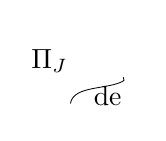
\begin{tikzpicture}[x=0.008cm,y=-0.008cm,baseline=(pide.base)]
\path[use as bounding box] (0,0) rectangle (175,135);
\node[anchor=base west,inner sep=0pt,outer sep=0pt] at (6,65) {\inserted{$\Pi_J$}};
\node[anchor=base west,inner sep=0pt,outer sep=0pt] (pide) at (105,124) {de};
\draw[line width=0.3pt,line cap=round] (68,120) .. controls (73,91) and (129,99) .. (153,84) -- (152,79);
\end{tikzpicture}
$X$ \deleted{definie} definie par les $\deleted{\unsure{\Sigma}}E_j$ $(j\in J)$, \unsure{\deleted{et}|et} \unsure{intersection|Intersection} des partitions
% G04: ternaires Pi_j insertion and its long bent caret. Source origin (970,1345).
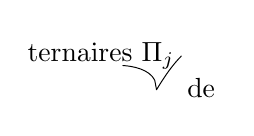
\begin{tikzpicture}[x=0.0075cm,y=-0.0075cm,baseline=(terde.base)]
\path[use as bounding box] (0,0) rectangle (335,135);
\node[anchor=base west,inner sep=0pt,outer sep=0pt] at (0,57) {\inserted{ternaires $\Pi_j$}};
\node[anchor=base west,inner sep=0pt,outer sep=0pt] (terde) at (270,118) {de};
\draw[line width=0.35pt,line cap=round,line join=round] (161,64) .. controls (177,65) and (206,70) .. (215,89) -- (218,105) .. controls (233,80) and (246,62) .. (260,48);
\end{tikzpicture}
$X$ $(j\in J)$ definies par les $E_j$ $\unsure{\deleted{\in}|\deleted{E}|\notin}$ $(j\in J)$
\[
X=E_j\amalg\coprod_{\alpha\in\pi_0(X\setminus E_j)}
% M03: detached short mark near the Sigma head and alpha. Dotless j avoids drawing an additional dot.
% Outer source origin (1145,1624); inner origin is explicitly translated to (1192,1627).
\begin{tikzpicture}[x=0.01cm,y=-0.01cm,baseline=(sigbase)]
\coordinate (sigbase) at (0,70);
\path[use as bounding box] (0,0) rectangle (110,88);
\begin{scope}[overlay]
\node[anchor=base west,inner sep=0pt,outer sep=0pt] at (0,70) {$\Sigma_{\jmath}^{\alpha}$};
\node[anchor=base west,inner sep=0pt,outer sep=0pt] at (47,3) {$\unsure{\begin{tikzpicture}[x=0.01cm,y=-0.01cm,baseline=(mthreebase)]
\coordinate (mthreebase) at (0,0);
\path[use as bounding box] (0,0) rectangle (7,7);
\fill (1,6) -- (0,4) -- (3,0) -- (5,1) -- (6,3) -- cycle;
\end{tikzpicture}}$};
\end{scope}
\end{tikzpicture}
\hspace{3cm}\raisebox{-0.45cm}{$\unsure{\begin{tikzpicture}[x=0.01cm,y=-0.01cm,baseline=(mtwobase)]
% M02a and M02b: source origin (1568,1738); two separate dark specks, with unestablished role and hand.
\coordinate (mtwobase) at (0,0);
\path[use as bounding box] (0,0) rectangle (13,17);
\fill (8,3) -- (10,0) -- (12,3) -- (11,5) -- (8,6) -- cycle;
\fill (1,11) -- (4,10) -- (6,12) -- (3,15) -- (1,14) -- cycle;
\end{tikzpicture}}$}
\]

-- c'est aussi la partition definie par celle de
% G06: detached baseline point before the first union, role and hand unresolved.
$\displaystyle \unsure{\mathord{
\begin{tikzpicture}[x=0.025cm,y=-0.025cm,baseline=0pt]
\useasboundingbox (0,0) rectangle (9,7);
\begin{scope}[shift={(-734,-1902)}]
\fill (735,1903) -- (741,1902) -- (741,1907) -- (735,1907) -- cycle;
\end{scope}
\end{tikzpicture}}}\bigcup_{j\in J}E_j$ en les $E_j$, et la partition
% G07: raised Pi_J ring and bent guide; source origin (752,1973).
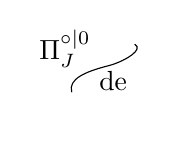
\begin{tikzpicture}[x=0.010cm,y=-0.010cm,baseline=(live.base)]
\useasboundingbox (0,0) rectangle (168,110);
\node[anchor=base west,inner sep=0pt,outer sep=0pt] (added) at (15,40) {\inserted{$\Pi_J^{\unsure{\circ|0}}$}};
\node[anchor=base west,inner sep=0pt,outer sep=0pt] (live) at (91,80) {de};
\begin{scope}[shift={(-752,-1973)}]
\draw[line width=0.40pt] (808,2055) .. controls (803,2038) and (826,2029) .. (852,2022) .. controls (870,2018) and (894,2005) .. (891,1997) -- (888,1994);
\end{scope}
\end{tikzpicture}
$\displaystyle X\setminus\mathop{\unsure{
\begin{tikzpicture}[x=0.01cm,y=-0.01cm,baseline=(unionbase)]
% G06: source origin (1115,1975); cup and visible transverse stroke; its mathematical role remains unassigned.
\coordinate (unionbase) at (0,58);
\path[use as bounding box] (0,0) rectangle (70,62);
\draw[line width=0.5pt,line cap=round] (14,4) .. controls (8,20) and (10,45) .. (26,54) .. controls (42,65) and (67,48) .. (65,22) .. controls (65,12) and (63,7) .. (61,4);
\draw[line width=0.5pt,line cap=round] (7,16) -- (56,14);
\end{tikzpicture}}}\limits_{j\in J}E_j$ intersection des partitions binaires $\Pi_{J,j}^{\circ}$
% The upper ring's local circle/zero doubt is recorded also at this second occurrence.
% G09: inserted (j in J), live induites, and one continuous hooked guide.
% Fixed source origin (1234,2070); the guide supplies no extra prose parenthesis.
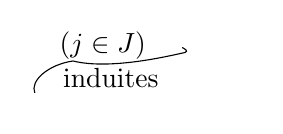
\begin{tikzpicture}[x=0.009cm,y=-0.009cm,baseline=(live.base)]
\useasboundingbox (0,0) rectangle (320,110);
\node[anchor=base west,inner sep=0pt,outer sep=0pt] (added) at (45,35) {\inserted{$(j\in J)$}};
\node[anchor=base west,inner sep=0pt,outer sep=0pt] (live) at (50,84) {induites};
\begin{scope}[shift={(-1234,-2070)}]
\draw[line width=0.40pt] (1244,2162) .. controls (1237,2145) and (1263,2122) .. (1298,2117) .. controls (1350,2130) and (1433,2110) .. (1456,2105) .. controls (1461,2103) and (1456,2100) .. (1452,2098);
\end{scope}
\end{tikzpicture}
% G10: U-subscript correction states and its long guide into the sur/X gap.
% Fixed source origin (311,2140); glyph/state alternatives carry no chronology.
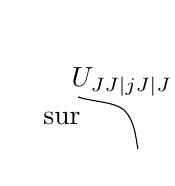
\begin{tikzpicture}[x=0.010cm,y=-0.010cm,baseline=(live.base)]
\useasboundingbox (0,0) rectangle (151,165);
\node[anchor=base west,inner sep=0pt,outer sep=0pt] (added) at (56,75) {\inserted{$U_{\unsure{\deleted{J}J|\deleted{j}J|J}}={}$}};
\node[anchor=base west,inner sep=0pt,outer sep=0pt] (live) at (20,123) {sur};
\begin{scope}[shift={(-311,-2140)}]
\draw[line width=0.40pt] (375,2228) .. controls (392,2234) and (422,2234) .. (434,2245) .. controls (447,2259) and (448,2277) .. (451,2294);
\end{scope}
\end{tikzpicture}
$\displaystyle X\setminus\bigcup_{j\in J}E_j$ par les $\Pi_j$ $(\unsure{g|j}\in J)$. Pour
% archive sheet number: 16
